\chapter{KẾT QUẢ NGHIÊN CỨU} \label{sec:chapter_3}
\section{Phương pháp tiếp cận}
\subsection{Hệ thống VLC}
\begin{figure} [H]
	\centering
	\captionsetup{justification=centering}
	\includegraphics [scale=0.5]
	{ThuPhat.png}
	\caption{Hệ thống \ac{vlc} thực tế tại phòng thí nghiệm 209B1}
\end{figure}
\begin{table}[H]
	\caption{Bảng các thành phần của hệ thống VLC thực tế}.
	\begin{center}
		\small
		\begin{tabular}{|c|c|}
			\hline
			Thiết bị & Thông số\\
			\hline
			\multirow{2}{*}{Generator AFG 3152C}
			&Tốc độ lấy mẫu tối đa 1GS/s, 2 kênh, băng thông 150MHz\\
			&Có thể phát dạng sóng Sine, Square, Pulse, Ramp, Guassian,…. \\			
			&Điều chế AM, FM, PM, FSK, PWM \\
			&Nguồn 100 - 240 V, 47 - 63 Hz\\
			\hline
			\multirow{2}{*}{Oscilloscope}
			&Tốc độ lấy mẫu tối đa 1GS/s\\
			&Băng thông 50MHz\\ 
			&Void/Div tối thiểu 2mV\\
			\hline
			\ac{oled} & Băng thông khoảng 4.3kHz\\
			\hline
			\multirow{2}{*}{Photodiode (PD)}
			& PDA36A của ThorLab \\
			& Bước sóng từ 350 – 1100 nm \\
			& Độ lợi tùy chỉnh từ 0 đến 70 dB \\
			& Điện áp tối đa 5 V và trở kháng 50 $\Omega$ \\
			\hline
			\multirow{2}{*}{Nguồn DC}
			& Điện áp 1.1 - 1.3 V \\
			& Cường độ dòng điện 0.7 - 0.9 A \\
			\hline
		\end{tabular}
		\label{tab:VLC_info}
	\end{center}
\end{table}
\newpage
\subsection{Dữ liệu}
Dữ liệu được sử dụng trong bài toán này là tín hiệu \ac{nrz} thu được từ photodiode. Tín hiệu thu được trong khoảng tần số từ 40kHz đến 63kHz, khoảng cách từ 25 cm đến 150 cm. Mỗi chuỗi thu được từ Ocsiloscope
bao gồm 2500 điểm.

Để đánh giá tín hiệu thu được một cách tổng quát, chúng ta dùng thông số là BER được tính dựa trên SNR. SNR được tính dựa trên giản đồ mắt, có giá trị bằng:
\begin{equation}
	SNR  = \frac{mean(highlevel) - mean (lowlevel)}{\sigma(highlevel) + \sigma(lowlevel)}
\end{equation}
Công thức trên được tính theo V, nên cần đổi ra dB bằng cách lấy $20\log_{10}$ kết quả ở trên.

\ac{ber} được tính theo công thức sau:
\begin{equation}
	BER = \frac{1}{2} erfc (\sqrt{SNR})
\end{equation}
Đây chính là số bit lỗi được ước lượng dưa trên tín hiệu thu được mà chưa qua mạng nơ-ron. Mục tiêu của chúng ta là cải thiện khả năng phân loại của mạng dựa vào mạng nơ-ron.

Dữ liệu thu được qua nhiều lần đo sau khi thu được chuẩn hóa về khoảng [0,1] dựa vào min-max normalization. Việc này làm tránh sự khác biệt về công suất do mỗi lần đo điều được chỉnh điện áp bằng tay.
Dựa trên 2500 sample thu được ở Ocsiloscope tách các sample ứng với 1 symbol truyền đi và gán nhãn. Sau đó tiến hành phân loại dựa trên mạng nơ-ron xác suất.
\begin{figure} [H]
	\centering
	\captionsetup{justification=centering}
	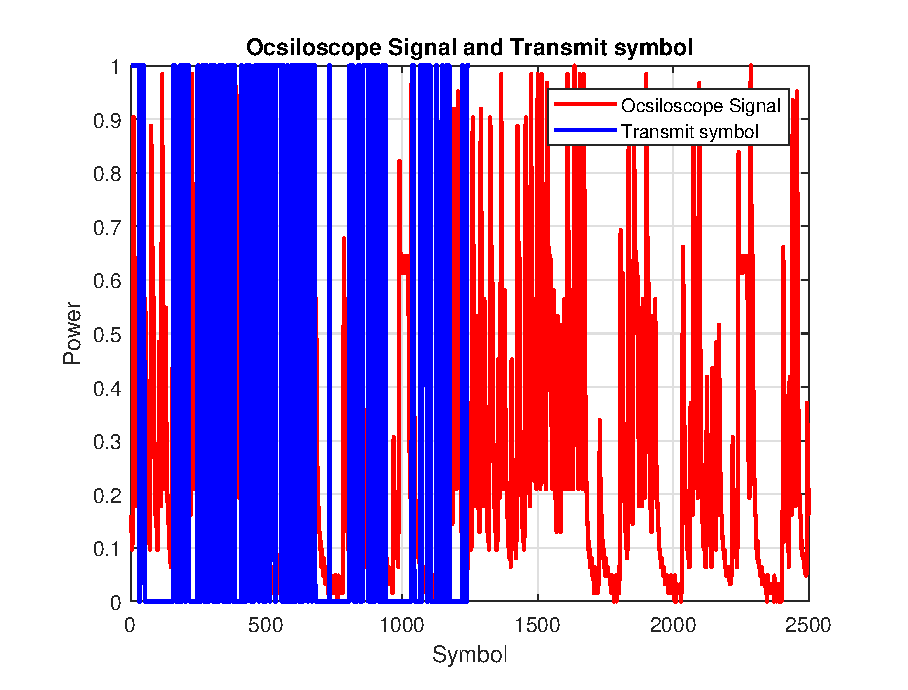
\includegraphics [scale=0.7]
	{ocsiloscope.eps}
	\caption{Tính độ tương quan giữa chuỗi phát và chuỗi thu}
	\label{fig:ocsiloscope}
\end{figure}
Dựa vào Hình \ref{fig:ocsiloscope}, ta có màu đỏ là tín hiệu sau khi thu đươc ocsiloscope đã chuẩn hóa công suất và màu xanh là tín hiệu truyền đi. Trong tín hiệu thu được ở ocsiloscope bao gồm tín hiệu truyền đi được lặp lại. Mục tiêu của chúng ta là xác định được điểm bắt đầu của tín hiệu và tách tín hiệu thu ứng với tín hiệu ta truyền đi. Ở đây ta có mỗi tín hiệu thu được là 2500 sample và cần ít nhất 2 tín hiệu truyền đi trên 1 tín hiệu thu để có thể tách được tín hiệu thu ứng với tín hiệu truyền. Trong báo cáo này chúng em chọn 5 sample và 250 symbol cho 1 tín hiệu.
Sau khi thu được tín hiệu. Dựa vào chuỗi truyền đi mà chúng ta tính độ tương quan bằng cách tính độ tương quan qua các lần dịch phải cho đến khi kết thúc tín hiệu thu. Kết quả sau khi tách chuỗi thu theo độ tương quan như Hình \ref{fig:ocsiloscope}.

\begin{figure}
	\centering
	\captionsetup{justification=centering}
	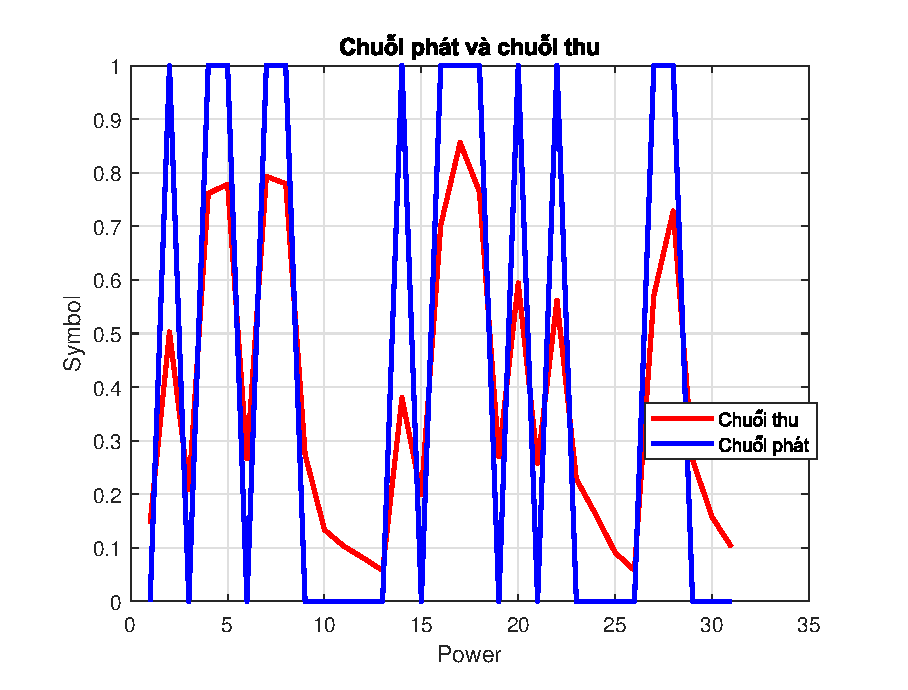
\includegraphics [scale=0.7]
	{transandreceive.eps}
	\caption{Độ tương quan giữa chuỗi phát và chuỗi thu}
	\label{fig:TransandReceive}
\end{figure}
\subsection{Ứng dụng mạng nơ-ron xác suất}
Trong đề tài luận văn này, tín hiệu được sử dụng là tín hiệu NRZ 2 mức 0 và 1,sau khi đi qua hệ thống sẽ bị biến đổi thành tín hiệu có các mức khác nhau. Bài toán đặt ra ở bộ cân bằng là làm thế nào để biến đổi các mức tín hiệu khác nhau về thành tín hiệu ban đầu có 2 mức 0 và 1. Để đánh giá tổng quan dữ liệu trước khi training có thể xem biểu đồ mắt như Hình \ref{fig:eye}.

\begin{figure}
	\centering
	\captionsetup{justification=centering}
	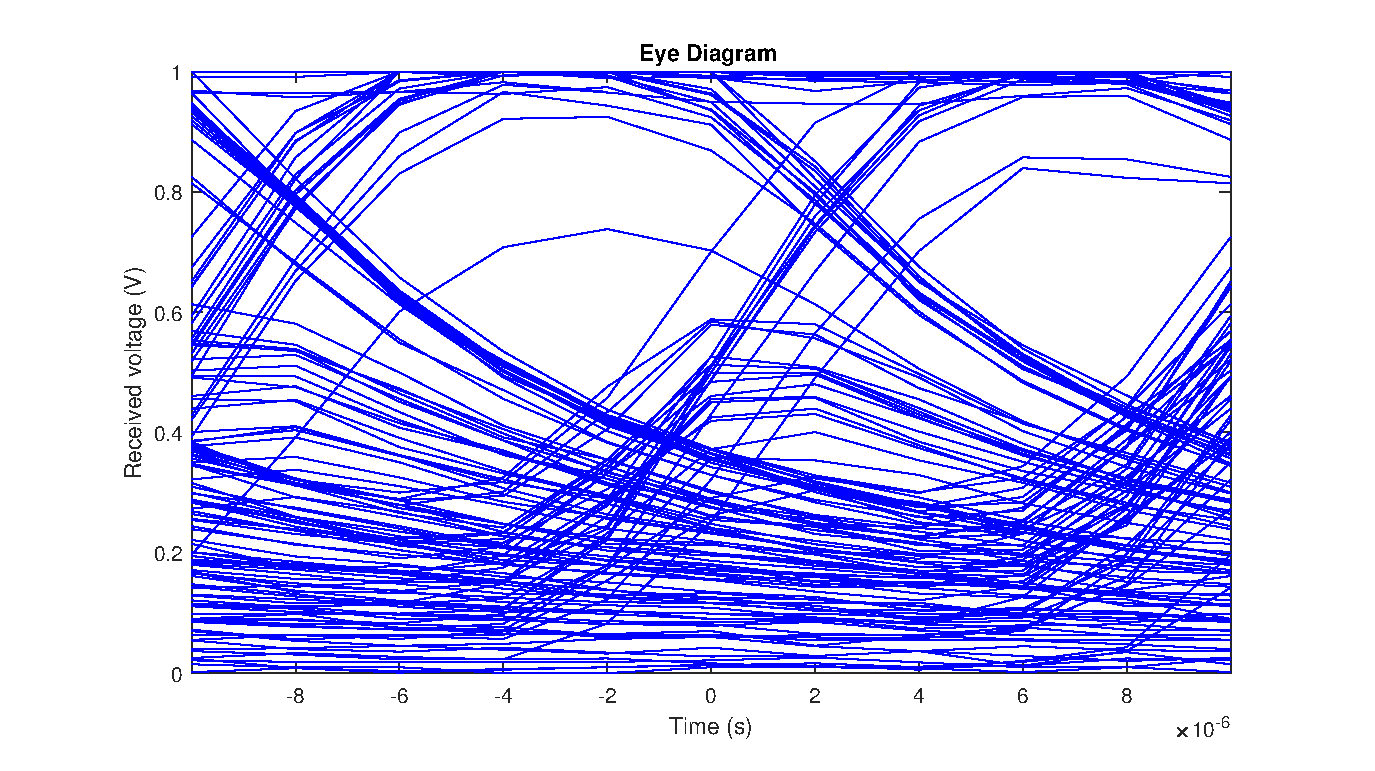
\includegraphics [scale=0.7]
	{eye.eps}
	\caption{Biểu đồ mắt}
	\label{fig:eye}
\end{figure}

Dựa vào \cite{eyediagram}, khi truyền ở tốc độ cao, chuỗi thu có gần như không xác định được độ mở mắt nên khó có thể phân loại được dữ liệu dựa vào mắt thường. Vì vậy mà chúng em quyết định bài toán phân lớp nên chúng em quyết định chọn mạng nơ-ron xác suất đề giải quyết vấn đề. Ngoài ra còn 1 điểm nữa là mô hình \ac{pnn} là 1 hàm có sẵn trong matlab mà còn rất tối ưu nên rất thuận tiện cho việc xử lý chuỗi tín hiệu lên đến hàng ngàn bit. Dựa vào chuỗi thu độ tương quan đã đề cập ở trên. Chúng ta chia nhỏ chuỗi thành các bit với nhãn '0' và '1' và tiến hành training bằng mạng nơ-ron xác suất. Từ đó đưa ra đánh giá đối với mô hình.


\newpage
\section{Kết quả và phân tích}
\subsection{Khảo sát sự ảnh hưởng của tốc độ bitrate}
Như đã đề cập, khi truyền ở tốc độ càng cao thì càng gây ra méo dạng phi tuyến. Mục tiêu trong khảo sát này là tìm ra được tốc độ truyền tối ưu có thể nhận biết được bằng mạng nơ-ron. Mục tiêu BER của khảo sát này là: 
 \begin{equation}
 	BER < 3.8*10^{-3}
 \end{equation}
Ta tiến hành khảo sát việc train và test dùng model PNN ở khoảng cách đo là 25cm ở các tốc độ bitrate: 40000,45000,50000,53000,55000,57000,60000,63000. Và xem xét sự thay đổi đổi BER. Từ đó ta có được đồ thị như Hình \ref{fig:BER}.

\begin{figure} [H]
	\centering
	\captionsetup{justification=centering}
	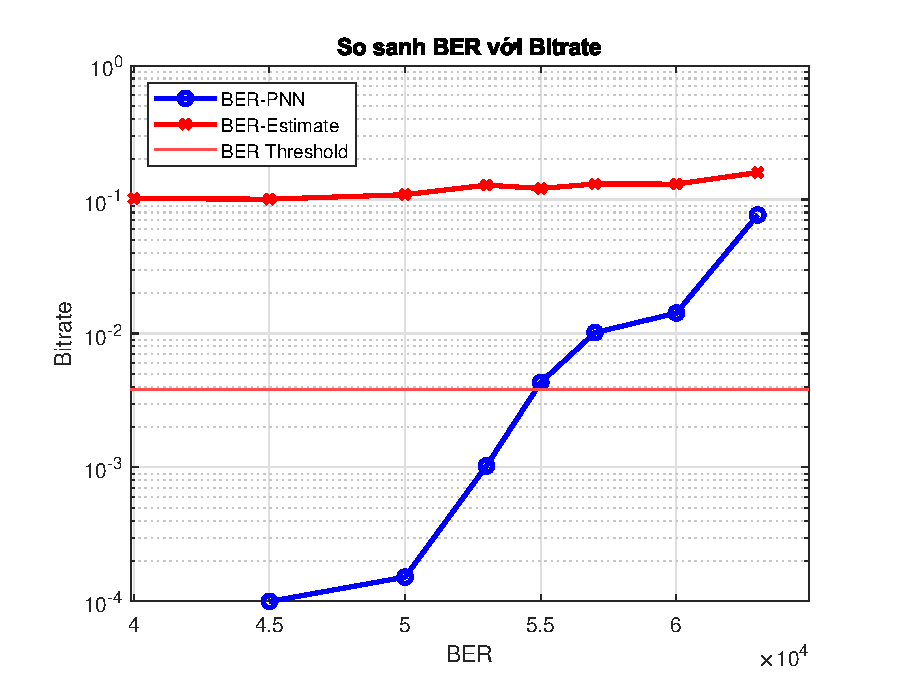
\includegraphics [scale=0.7]
	{BER.eps}
	\caption{So sánh BER giữa ước lượng và PNN}
	\label{fig:BER}
\end{figure}

Nhận xét: Từ đường màu đỏ có thể thấy BER mà chúng ta ước lượng dựa vào SNR gần như không đổi trên khoảng mà chúng ta khảo sát. Tuy nhiên khi sau khi sử dụng PNN thì giảm rõ rệt. Xét trên ngưỡng cắt BER thì ta có thể phân biệt được tín hiệu ở mức khoảng 54000.

\subsection{Khảo sát sự ảnh hưởng của số sample}
Xuất phát dựa trên việc cắt chuỗi các bit '0' và '1'. Việc tách chuỗi thu được tính dựa vào tương quan so với chuỗi phát. Việc lấy mẫu quá ít cũng có thể gây lệch chuỗi. Mục đích của khảo sát là tạo ra tập dữ liệu có độ tin cậy cao hơn để phân loại. Ngoài ra, việc tăng số sample có thể làm tăng số dữ liệu input. Việc này tuy làm chậm khả năng tính toán nhưng tăng tính ràng buộc của dữ liệu. Từ đó mà cho ta kết quả phân loại đúng hơn.




